\chapter{Tecnologie utilizzate}
Sono elencate ora le principali tecnologie utilizzate nel progetto. Alcune di esse avranno un ruolo prioritario in capitoli specifici.

\section{Android}
\begin{wrapfigure}{r}{0.1\textwidth}

\includegraphics[width=0.1\textwidth]{android-logo}
\end{wrapfigure} 
\FloatBarrier
Come vedremo nel capitolo ad esso dedicato, Android è più di un semplice linguaggio. Esso è infatti un ecosistema che unisce linguaggi di programmazione differenti con un sistema operativo sviluppato prettamente per dispositivi portatili.
Android nel caso specifico di questo progetto è l'ambiente di sviluppo utilizzato per dare vita al client.

\section{ASP.Net}
\begin{wrapfigure}{r}{0.2\textwidth}

\includegraphics[width=0.2\textwidth]{asp-logo}
\end{wrapfigure} 
\FloatBarrier
Sulle tecnologie ASP.Net si basa l' "anima" dell'applicazione: il server.
ASP.Net non è semplicemente un linguaggio di programmazione, ma un insieme di tecnologie di sviluppo software per il web commercializzate da Microsoft.
Come tutte le applicazioni della famiglia Microsoft.NET si basa sul Common Language Runtime (CLR): ovvero gli sviluppatori possono scrivere codice in uno dei qualsiasi linguaggi supportati (Visual Basic .Net, C\#, J\#, Python e molti altri) che verrà poi interpretato automaticamente.
Nello specifico è stato utilizzato il pattern Model-View-Controller (MVC) che approfondiremo nel paragrafo relativo al server.

\section{HttpS}
\begin{wrapfigure}{r}{0.2\textwidth}
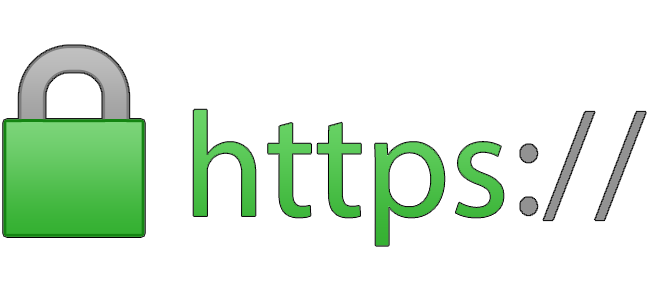
\includegraphics[width=0.2\textwidth]{https-logo}
\end{wrapfigure} 
\FloatBarrier
L' HyperText Transfer Protocol (protocollo di trasferimento di un ipertesto) è , appunto, un protocollo usato come principale sistema per la trasmissione d'informazioni sul web e quindi su architetture client-server.
La "S" identifica la connessione criptata dal Transport Layer Security (TLS) o dal suo predecessore Secure Sockets Layer (SSL) che ne garantisce l'integrità.
Https lavora al livello più alto del modello TCP\footnote{Transmission Control Protocolo (TCP), protocollo a livello di rete che  rende affidabile la comunicazione dati tra mittente e destinatario.}/IP, il livello di applicazione. In pratica, tra il protocollo TCP e Http si interpone un livello di crittografia/autenticazione che cripta il messaggio Http prima della trasmissione e lo decripta una volta arrivato a destinazione. In pratica viene stabilita una connessione criptata tra client e server tramite lo scambio di certificati che attestano l'identità delle due controparti.

\section{OAuth}
\begin{wrapfigure}{r}{0.2\textwidth}

\includegraphics[width=0.2\textwidth]{oauth-logo}
\end{wrapfigure} 
\FloatBarrier
OAuth è un protocollo che permette l'autorizzazione di API\footnote{Con Application Programming Interface (API) si indica ogni insieme di procedure disponibili al programmatore, di solito raggruppate a formare un set di strumenti specifici per l'espletamento di un determinato compito all'interno di un certo programma. Spesso con tale termine si intendono le librerie software disponibili in un certo linguaggio di programmazione.} di sicurezza con un metodo standardizzato e semplice per ogni tipo di applicazione, sia esso mobile o fisso. Questo sistema permette ai service providers, ovvero i fornitori di servizi che fanno uso di questo protocollo, di condividere informazioni specifiche dei propri utenti con servizi terzi proteggendone le credenziali (per esempio la password).
Per capirne il funzionamento prendiamo come esempio il caso di login ad un qualsiasi sito web tramite account Facebook:
\begin{enumerate}
\item L'utente accede al sito e avvia la procedura di login tramite Facebook
\item L'utente inserisce le sue credenziali per garantire l'accesso alle sue informazioni
\item Il service provider (Facebook) risponde con un Access Token univoco
\item Il sito web utilizzerà l'Access Token per accedere alle informazioni dell'utente senza saperne le credenziali
\end{enumerate}